\chapter{Simulation: Event Generation and Propagation}
\label{ch:simulation}
%SUPER MOOIE AFBEELDINGEN \url{http://www.hap-astroteilchen.de/poPAHrt.php}
\begin{flushright}
\textit{\\Soon there will be virtual reality, and augmented reality. If you assume any rate of improvement at all, then games will become indistinguishable from reality . . ., it would seem to follow that the odds we are in base reality are one in billions. $\sim$ Elon Musk\\}
\end{flushright}
To be able to search for new physics, one needs a good handle on the detector response to known physics processes. Depending on the analysis, some processes are more interesting than others. In general, the particle interactions of interest are referred to as \textit{signal events}. Other interactions, which mimic or obscure the signal events, are typically called \textit{background events}. These events are simulated using Monte Carlo\footnote{While recovering from an illness in 1946, Stanislaw Ulam figured that the actual counting of succesful attempts in playing a card game would yield him a much faster answer to the probability of succes rather than doing the actual calculus. His work, shared with John von Neumann, needed to remain secret and adopted the code word ``Monte Carlo''\index{Monte Carlo}, referring to the gambling games in the Monte Carlo Casino in Monaco.} (MC) simulations, where one makes use of a model that describes the interactions and their probability to occur. A typical MC simulation consists of hundreds to millions of events that are constructed using these models with the use of random number generators. To determine the detector response to a particle interaction, one first has to start with the particle generation, which sets the conditions of the initial interaction. Afterwards, the propagation of the particle in the detector (medium) is simulated as best as possible. Below, an overview of the important background and signal simulations that are used in this analysis is given. A flowchart of the simulations steps is shown in Figure \ref{fig:flowchart}.

\begin{figure}
\centering
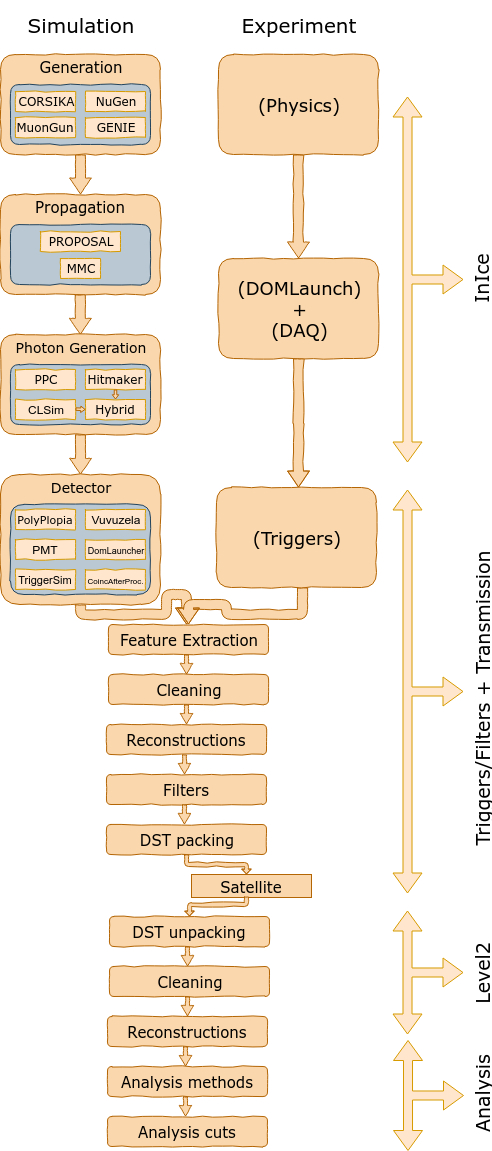
\includegraphics[width=0.65\textwidth]{chapter6/img/flowchart_extended.png}
\caption{Flowchart of the simulation layout. On the left is shown how particles are injected and their interactions are simulated down to digitized waveforms. The right part shows real data processing. After triggering, both data and simulation go through the same processing chain to prepare for analysis.}
\label{fig:flowchart}
\end{figure}

\section{The software framework}
\textit{IceTray} \index{IceTray} is a modular framework written and used by the IceCube collaboration and mostly written in C++ for fast computation. A Python interface for most modules is provided for fast and easy implementation of the code. The framework is used in both online and offline processing and is stream-based with modules that act on events in the stream and essentially follows a flowchart of modules that is provided by the user.\\

\noindent To process the large amount of simulation that is required for the collaboration, a data processing and management framework called \textit{IceProd} was developed. The setup is very light-weight, running as a Python application. It uses (complex) workflow DAGs (see below) across distributed computing grids in order to optimize usage of resources. A \textit{dataset} is set up by running hundreds to thousands of jobs in parallel over multiple computing resources all over the world. Each dataset has specific input parameters that are fixed. Distributions in physical parameters such as the direction, energy, position, etc. of the particle(s) are provided by random number generators \cite{1742-6596-664-6-062056}.\\

\noindent \textit{HTCondor} is an open source computing software that provides a job queueing mechanism, scheduling policy, priority scheme, resource monitoring, and resource management. Users submit their serial or parallel jobs to HTCondor which places them into a queue. It chooses when and where to run the jobs based upon a policy, carefully monitors their progress, and ultimately informs the user upon completion.\\

\noindent \textit{DAGMans} (Directed Acyclic Graph Managers) are meta-schedulers for the execution of computations. A Directed Acyclic Graph (DAG) consists out of nodes in a graph. Each node represents a certain computation that needs a certain input, output or execution that could depend on another node. Once a DAG is set up, DAGMans submit the programs to HTCondor in an order represented by a DAG an processes the results. DAGMans are often used by analyzers for bulk computations on large amounts of data.

\section{Generation}
Simulations start with setting up the starting conditions of the physical processes one wants to simulate. For example, a shower event by itself is not well defined. The type of primary particle (H, He, Fe,...), the energy, the inclination and so on will all determine the properties of the full air shower that is produced. Multiple different generators used in the IceCube collaboration serve different purposes; some are explained in more detail below.

\subsection{Background simulation}
In this work we search for signal events that are not exected from the Standard Model. However, the IceCube neutrino observatory is not designed to look for particles with an anomalous charge. Therefore, it is necessary to properly account the other physical processes that are not sought for in this analysis but can mimic the signature of the signal. SMPs with a charge lower than the electron charge will produce less light compared to muons due to the squared charge dependency in the Cherenkov effect (see Eq. \ref{eq:franktamm}). Because the optical modules are located far away from each other, most of the light that is produced in tracks is lost. For this reason, there is a large uncertainty on the amount of Cherenkov photons that were produced when a track is seen in an event. Muons that originate from air shower events can produce dim tracks and are simulated with CORSIKA simulation. The NuGen program was used to simulate events originating from neutrinos. Both simulation programs are given in more detail below. The datasets used in this analysis use SpiceLea as the ice model (see Section \ref{subsec:icesimulation}). An overview of the data samples and several simulation paramaters is given in Table \ref{tab:datasets}

\subsubsection{CORSIKA}
\label{subsub:corsika}
A free, publicly available software framework that is widely used in the astrophysics community for the simulation of cosmic ray interactions is called CORSIKA \index{CORSIKA} (COsmic Ray SImulations for Kascade) \cite{Heck:1998vt}. It was originally developed for the KASCADE experiment and is now used by most people and collaborations to simulate air shower events. IceCube analyses, such as this one, use CORSIKA simulations to simulate the muonic component that is able to reach the in-ice detector.

The code is written in FORTRAN 77, but a C++ version is currently in the making \cite{Engel:2018akg}.\\

\noindent The program initially injects a particle of specific type, energy, direction and position in the top of the atmosphere. The particles are tracked through the atmoshpere until they undergo reactions with the air nuclei or - in the case of instable secondaries - decay. Multiple different hadronic interaction models exist to describe the interactions at high energies such as QGSJET \cite{Ostapchenko:2010vb}, SIBYLL \cite{Riehn:2017mfm} and EPOS-LHC \cite{Pierog:2013ria}. The production of new particles after decay or interaction creates showers of particles and these particles are saved and read out at a certain altitude. Because the flux of cosmic rays is exceedingly small at the highest energies, too many resources and too much time would be required to simulate an energy distribution as measured in experiments. Therefore, one often simulates a much harder spectrum and reweights the events accordingly later on (see Section \ref{sec:weighting}). Simulation datasets are often subdivided into a low-energy and high-energy dataset. In this analysis, the former ranges from primary energies between 600 GeV to 100 TeV and uses a spectral index that is close to what is measured ($\gamma = 2.6$). The spectral index of the latter is smaller, resulting in a harder spectrum ($\gamma = 2$) leading to more statistics for rare high-energy events. The primary energy ranges from 100 TeV to 100 EeV. The lower limit of the energy range at 600 GeV is due to the limited penetration depth of muons through the ice.\\

\noindent The spectrum used for this analysis, after reweighting, follows the following energy distribution:

\begin{equation}
\label{eq:gaisser}
\Phi_i \left(E_{\textrm{prim}}\right) = \sum^3_{j=1} a_{i,j} E^{-\gamma_{i,j}} \cdot \exp \left[- \frac{E}{Z_i R_{c,j}}\right].
\end{equation}

\noindent where we sum over three populations: particles accelerated from supernova remnants, a higher-energy galactic component of unknown origin and particles accelerated to ultra-high-energy from extra-galactic sources (more info in Section \ref{subsubsec:galactic}). $\gamma$ is the spectral index, $Z$ the particle atomic number and $a_{i,j}$ the normalization constants for primary $i$ in population $j$. $R$ is the magnetic rigidity and $R_c$ is the characteristic rigidity or cutoff above which a particular acceleration process reaches its limit. The 5 groups that are assumed to contribute significantly to the flux are: p, He, CNO, Mg-Si and Fe. This is the convention that is used in Ref. \cite{Gaisser:2013bla}. Table \ref{tab:fluxnormalization} summarizes the typical values for these parameters and shows the best fits for the normalization constants to describe the data.

\begin{table}[]
\centering
\caption{Best fit for parameters in Eq. \ref{eq:gaisser}. Numbers taken from Ref. \cite{Gaisser:2013bla}.}
\label{tab:fluxnormalization}
\resizebox{\textwidth}{!}{%
\begin{tabular}{|c|c|c|c|c|c|c|c|c|c|c|c|}
\hline
\cellcolor[HTML]{F1A91E}$j$ & \cellcolor[HTML]{F1A91E}$R_c$ {[}V{]} & \multicolumn{5}{c|}{\cellcolor[HTML]{F1A91E}$\gamma$} & \multicolumn{5}{c|}{\cellcolor[HTML]{F1A91E}$a_{i,j}$} \\ \hline
 &  & p & He & CNO & Mg-Si & Fe & p & He & CNO & Mg-Si & Fe \\ \hline
1 & $4 \cdot 10^{15}$ & 1.66 & 1.58 & 1.63 & 1.67 & 1.63 & 7860 & 3550 & 2200 & 1430 & 2120 \\ \hline
2 & $30 \cdot 10^{15}$ & \multicolumn{5}{c|}{1.4} & \multicolumn{2}{c|}{20} & \multicolumn{3}{c|}{13.4} \\ \hline
3 & $2 \cdot 10^{18}$ & \multicolumn{5}{c|}{1.4} & \multicolumn{2}{c|}{1.7} & \multicolumn{3}{c|}{1.14} \\ \hline
\end{tabular}%
}
\end{table}

\paragraph{Interactions}
The atmosphere composition is always set at 78.1\% N$_2$, 21\% O$_2$, and 0.9\% Ar, which is a good description of reality. However, the density of the air above the detector changes significantly during the year because of temperature differences in the Antarctic summer and winter. Most analyses, including this one, treat the muonic component as a background and are not interested in the details of the showers and how it changes during the year and therefore use an average of the atmospheric density. The atmospheric depth and densities were set to the averages of the month November for 5 years of data \cite{samDeRidder}. This is shown in Figure \ref{fig:atmosphere}.\\

\begin{figure}
\centering
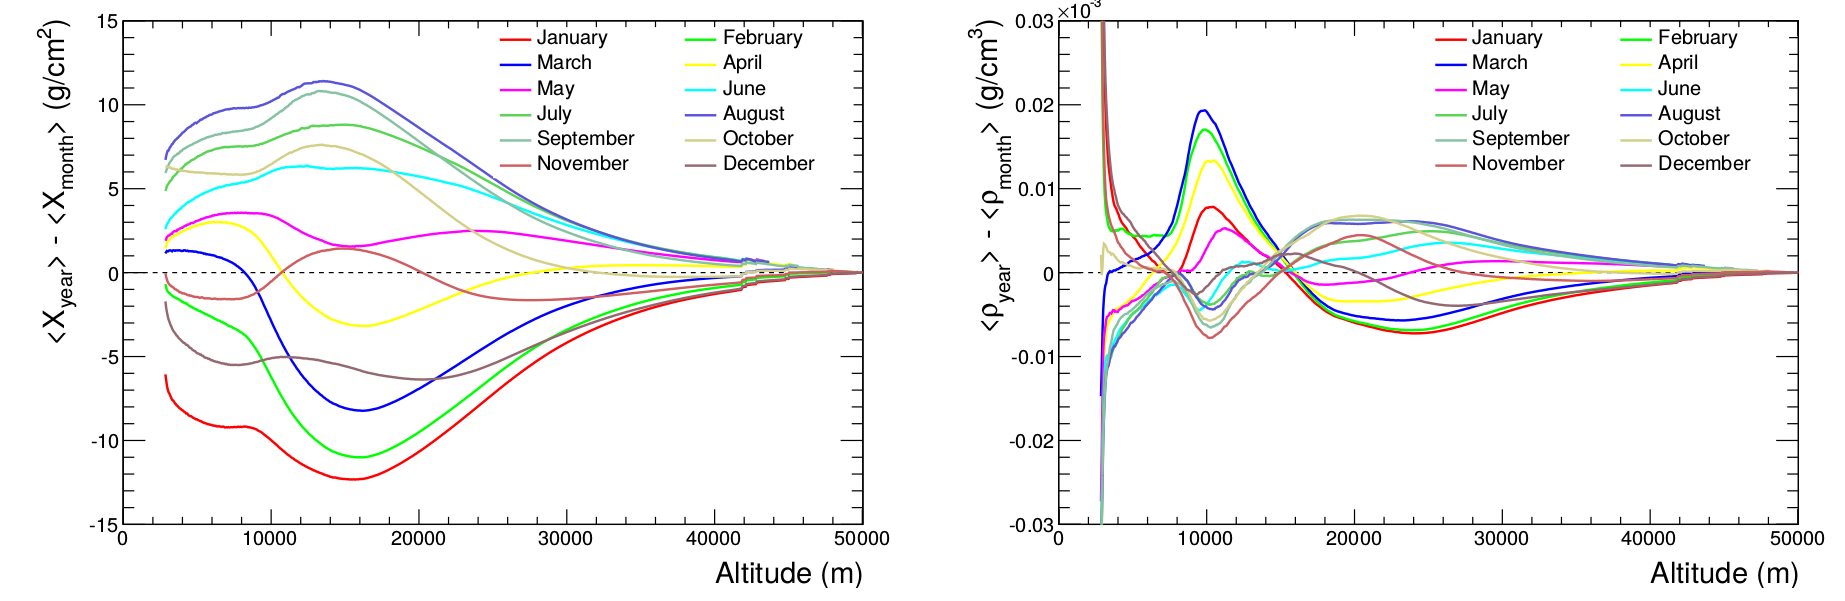
\includegraphics[width=\textwidth]{chapter6/img/atmosphere.png}
\caption{\textit{Left: }Average atmospheric depth per month. \textit{Right: }Average atmospheric density per month. Figures obtained with 5 years of data (2007-2011) \cite{samDeRidder}.}
\label{fig:atmosphere}
\end{figure}

\noindent The shower propagation and composition depends on the models that are used to simulate the high-energy interactions. The lowest energies are simulated with FLUKA \index{FLUKA} (FLUktuierende KAskade) \cite{Battistoni:2015epi}. This model covers the energy range that can be compared with accelerator experiments.  The SIBYLL model was used for the high-energy interactions. However, which model is the best for the highest energies is not known at the time of writing since there are no controlled laboratory measurements that are capable of reaching these energies. Several studies seem to indicate that the composition changes drastically at the highest energies, i.e. IceCube \cite{Rawlins:2016bkc}, Pierre Auger Observatory \cite{Porcelli:2015jli}, and Telescope Array \cite{Belz:2015cvi}. However, the different experiments do not agree, presumably due to the different techniques used to determine the primary composition \cite{samDeRidder}. Recent work has shown that the most likely cause of discrepency lies in non-perfect models \cite{Dembinski:2019uta}. Even though this discussion is far from resolved, it is fortunately of no importance for this analysis as these effects become more prominent at the higher energies.\\

\subsubsection{NuGen}
\label{subsec:nugen}
The neutrino-generator\index{neutrino-generator} (NuGen) is a neutrino event generator program that works with the IceTray framework. With this module, one can inject a primary neutrino on the surface of the Earth by specifying a few parameters in the steering file.

The physics implemented in this program is based on the ANIS-All Neutrino Interaction Generator \cite{Gazizov:2004va}. However, the cross sections have been updated and the structure of the code has been changed significantly from ANIS to incorporate it in the IceTray framework.\\

\noindent The generator requires the first interaction to be near the detector and

\newcommand\barparen[1]{\overset{(-)}{#1}}
\vspace{2mm}
\begin{itemize}
\item prepares a primary neutrino and injects it to the Earth,
\item propagates the neutrino and works out interactions inside the Earth\footnote{Possible interactions are CC, NC, Glashow resonance for $\bar{\nu}_e$ and $\tau$ decay for $\barparen{\nu_\tau}$. CC interactions produce no new neutrinos and the simulation stops at the vertex point. The other interactions create new secondary neutrinos.} (when they occur),
\item makes a forced interaction inside the detection volume\footnote{
In most cases, a neutrino will not interact within the medium, but for computational reasons at least one neutrino is forced to interact and the simulation is reweighted afterwards accordingly.} (only if any neutrino reaches the detector site),
\item stores injected neutrinos and all generated secondaries,
\item stores interaction weight information.
\end{itemize}
\vspace{3mm}
\noindent The generator alternates between neutrino and antineutrino and assumes a neutrino-antineutrino ratio of (1:1).\\

\noindent The spectrum used for this analysis, after reweighting, follows the Honda2006 spectrum \cite{Honda:2006qj} for atmospheric neutrinos, SarcevicStd for the prompt component \cite{Enberg:2008te}, and an astrophysical flux fit from Ref. \cite{Aartsen:2014gkd} (see Section \ref{sec:neutrinos} for more information on these fluxes). The astrophysical flux measured by the IceCube collaboration follows an energy spectrum equal to

\begin{equation}
E^2 \left(\Phi \right) = 1.5 \cdot 10^{-8} \left( \frac{E}{100 \textrm{ TeV}} \right)^{-0.3} \textrm{GeV } \textrm{cm}^{-2} \textrm{s}^{-1} \textrm{sr}^{-1}.
\end{equation}
\vspace{3mm}
\noindent The distribution for these different components can be seen in Figure \ref{fig:neutrinospectrum}.

\begin{figure}
\centering
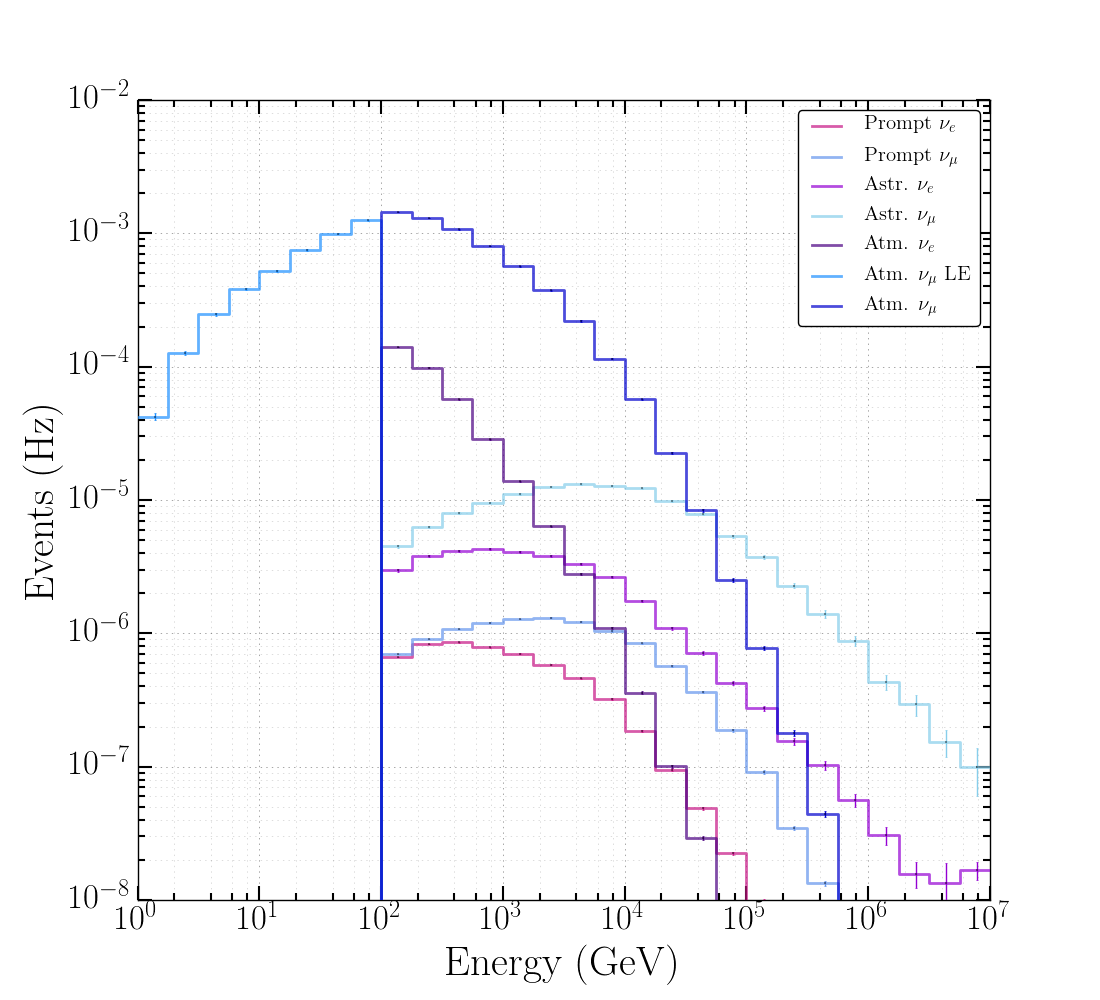
\includegraphics[width=0.6\textwidth]{chapter6/img/neutrinoenergy.png}
\caption{Distribution of weighted neutrino fluxes that were used for this analysis. The atmospheric $\nu_\mu$ and $\nu_e$ fluxes were derived from Ref. \cite{Honda:2006qj}, prompt from Ref. \cite{Enberg:2008te}, and astrophysical from Ref. \cite{Aartsen:2014gkd}. The energy refers to the energy of the primary neutrino.}
\label{fig:neutrinospectrum}
\end{figure}

\subsubsection{GENIE}
To include the lowest energies (0.5 - 100 GeV), which are not included in ANIS/NuGen, the GENIE (Generates Events for Neutrino Interaction Experiments) neutrino generator was implemented in IceTray. It is a well established generator, used by collaborations worldwide and written in C++ \cite{Andreopoulos:2009rq,Andreopoulos:2015wxa}.\\

\noindent The spectrum used for this analysis, after reweighting, follows the Honda2015 spectrum \cite{Honda:2015fha} for low-energy atmospheric neutrinos.

\begin{table}[]
\centering
\small
\caption{Overview of the datasets used in this analysis. GaisserH3a from Ref. \cite{Gaisser:2013bla}, Honda2015 from Ref. \cite{Honda:2015fha}, Honda2006 from Ref. \cite{Honda:2006qj}, Sarcevic from Ref. \cite{Enberg:2008te}, and astrophysical from Ref. \cite{Aartsen:2014gkd}. The dataset number is a unique number used in IceProd to distinguish data samples.}
\label{tab:datasets}
\resizebox{\textwidth}{!}{%
\begin{tabular}{|l |c|c|c|c|c|r|}
\hline
\cellcolor[HTML]{F1A91E}Generator & \cellcolor[HTML]{F1A91E}Type & \cellcolor[HTML]{F1A91E}Range {[}GeV{]} & \cellcolor[HTML]{F1A91E}Simulated $\gamma$ & \cellcolor[HTML]{F1A91E}Weighted $\gamma$ & \cellcolor[HTML]{F1A91E}Ice & \cellcolor[HTML]{F1A91E}Dataset \\ \hline
\textbf{CORS.} & 5-comp. & $10^5 - 10^{11}$ & 2 & GaisserH3a & SpiceLea & 11937 \\ \hline
\textbf{CORS.} & 5-comp. & $600 - 10^5$ & 2.6 & GaisserH3a & SpiceLea & 11499 \\ \hline
\textbf{CORS.} & 5-comp. & $600 - 10^5$ & 2.6 & GaisserH3a & SpiceLea & 11808 \\ \hline
\textbf{CORS.} & 5-comp. & $600 - 10^5$ & 2.6 & GaisserH3a & SpiceLea & 11865 \\ \hline
\textbf{CORS.} & 5-comp. & $600 - 10^5$ & 2.6 & GaisserH3a & SpiceLea & 11905 \\ \hline
\textbf{CORS.} & 5-comp. & $600 - 10^5$ & 2.6 & GaisserH3a & SpiceLea & 11926 \\ \hline
\textbf{CORS.} & 5-comp. & $600 - 10^5$ & 2.6 & GaisserH3a & SpiceLea & 11943 \\ \hline
\textbf{CORS.} & 5-comp. & $600 - 10^5$ & 2.6 & GaisserH3a & SpiceLea & 12161 \\ \hline
\textbf{CORS.} & 5-comp. & $600 - 10^5$ & 2.6 & GaisserH3a & SpiceLea & 12268 \\ \hline
\textbf{GENIE} & $\nu_\mu$ & $0.5 - 100$ & 1 & Honda2015 & SpiceMie & 12475 \\ \hline
 &  &  &  & atmos.: Honda2006 &  &  \\
 &  &  &  & prompt: Sarcevic &  &  \\
\multirow{-3}{*}{\textbf{NuGen}} & \multirow{-3}{*}{$\nu_\mu$} & \multirow{-3}{*}{$100 - 10^8$} & \multirow{-3}{*}{2} & astro.: Astro. & \multirow{-3}{*}{SpiceLea} & \multirow{-3}{*}{11029} \\ \hline
 &  &  &  & atmos.: Honda2006 &  &  \\
 &  &  &  & prompt: Sarcevic &  &  \\
\multirow{-3}{*}{\textbf{NuGen}} & \multirow{-3}{*}{$\nu_\mu$} & \multirow{-3}{*}{$100 - 10^8$} & \multirow{-3}{*}{2} & astro.: Astro. & \multirow{-3}{*}{SpiceLea} & \multirow{-3}{*}{12346} \\ \hline
 &  &  &  & atmos.: Honda2006 &  &  \\
 &  &  &  & prompt: Sarcevic &  &  \\
\multirow{-3}{*}{\textbf{NuGen}} & \multirow{-3}{*}{$\nu_\mu$} & \multirow{-3}{*}{$100 - 10^8$} & \multirow{-3}{*}{2} & astro.: Astro. & \multirow{-3}{*}{SpiceLea} & \multirow{-3}{*}{11883} \\ \hline
 &  &  &  & atmos.: Honda2006 &  &  \\
 &  &  &  & prompt: Sarcevic &  &  \\
\multirow{-3}{*}{\textbf{NuGen}} & \multirow{-3}{*}{$\nu_e$} & \multirow{-3}{*}{$100 - 10^8$} & \multirow{-3}{*}{2} & astro.: Astro. & \multirow{-3}{*}{SpiceLea} & \multirow{-3}{*}{12034} \\ \hline
 &  &  &  & atmos.: Honda2006 &  &  \\
 &  &  &  & prompt: Sarcevic &  &  \\
\multirow{-3}{*}{\textbf{NuGen}} & \multirow{-3}{*}{$\nu_e$} & \multirow{-3}{*}{$100 - 10^8$} & \multirow{-3}{*}{2} & astro.: Astro. & \multirow{-3}{*}{SpiceLea} & \multirow{-3}{*}{12646} \\ \hline
\end{tabular}%
}
\end{table}

\subsection{Signal simulation}
As mentioned in Section \ref{sec:properties}, the signal flux is assumed to be isotropic close to the detector. The SMP starting points are randomly placed on a disk with a direction perpendicular to it as shown in Figure \ref{fig:injector}. The disk has a radius of 800 m and is located at a distance of 1000 m from the detector center. The disk itself is randomly rotated around the detector center to simulate an isotropic flux. The distribution of the azimuth, $\phi$, and cosine of the zenith\footnote{See Appendix \ref{sec:angularappendix} why we show the cosine of the zenith.}, $\cos(\theta)$, is shown in Figure \ref{fig:angles}.\\

\begin{figure}[t]
\centering
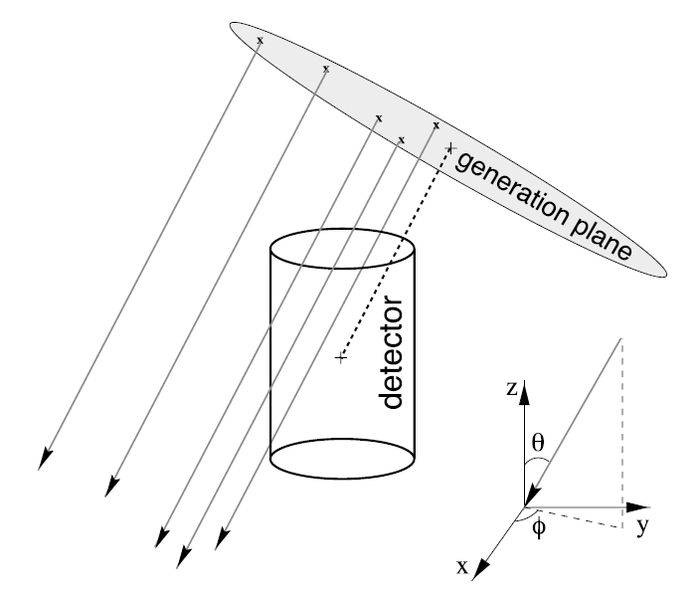
\includegraphics[width=0.5\textwidth]{chapter6/img/GenerationDisk.png}
\caption{Illustration of how the particle injection works. The particle is first randomly positioned on a disk following a uniform distribution. The disk is then randomly rotated to simulate an isotropic flux.}
\label{fig:injector}
\end{figure}

\begin{figure}[t]
\centering
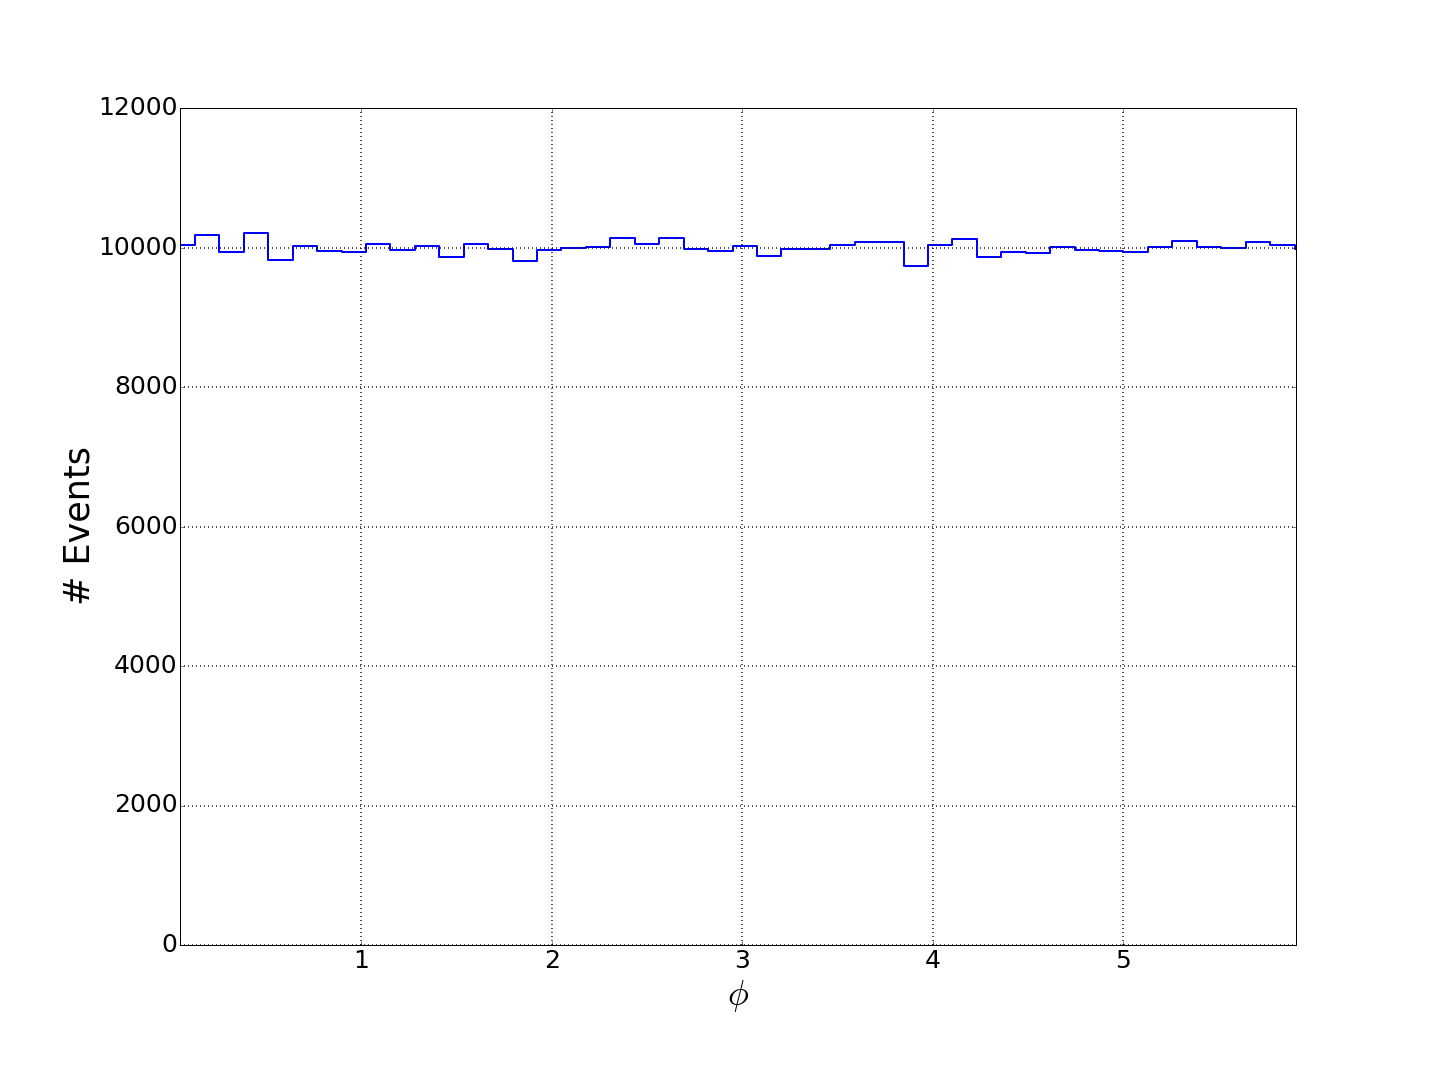
\includegraphics[width=0.49\textwidth]{chapter6/img/Azimuth}
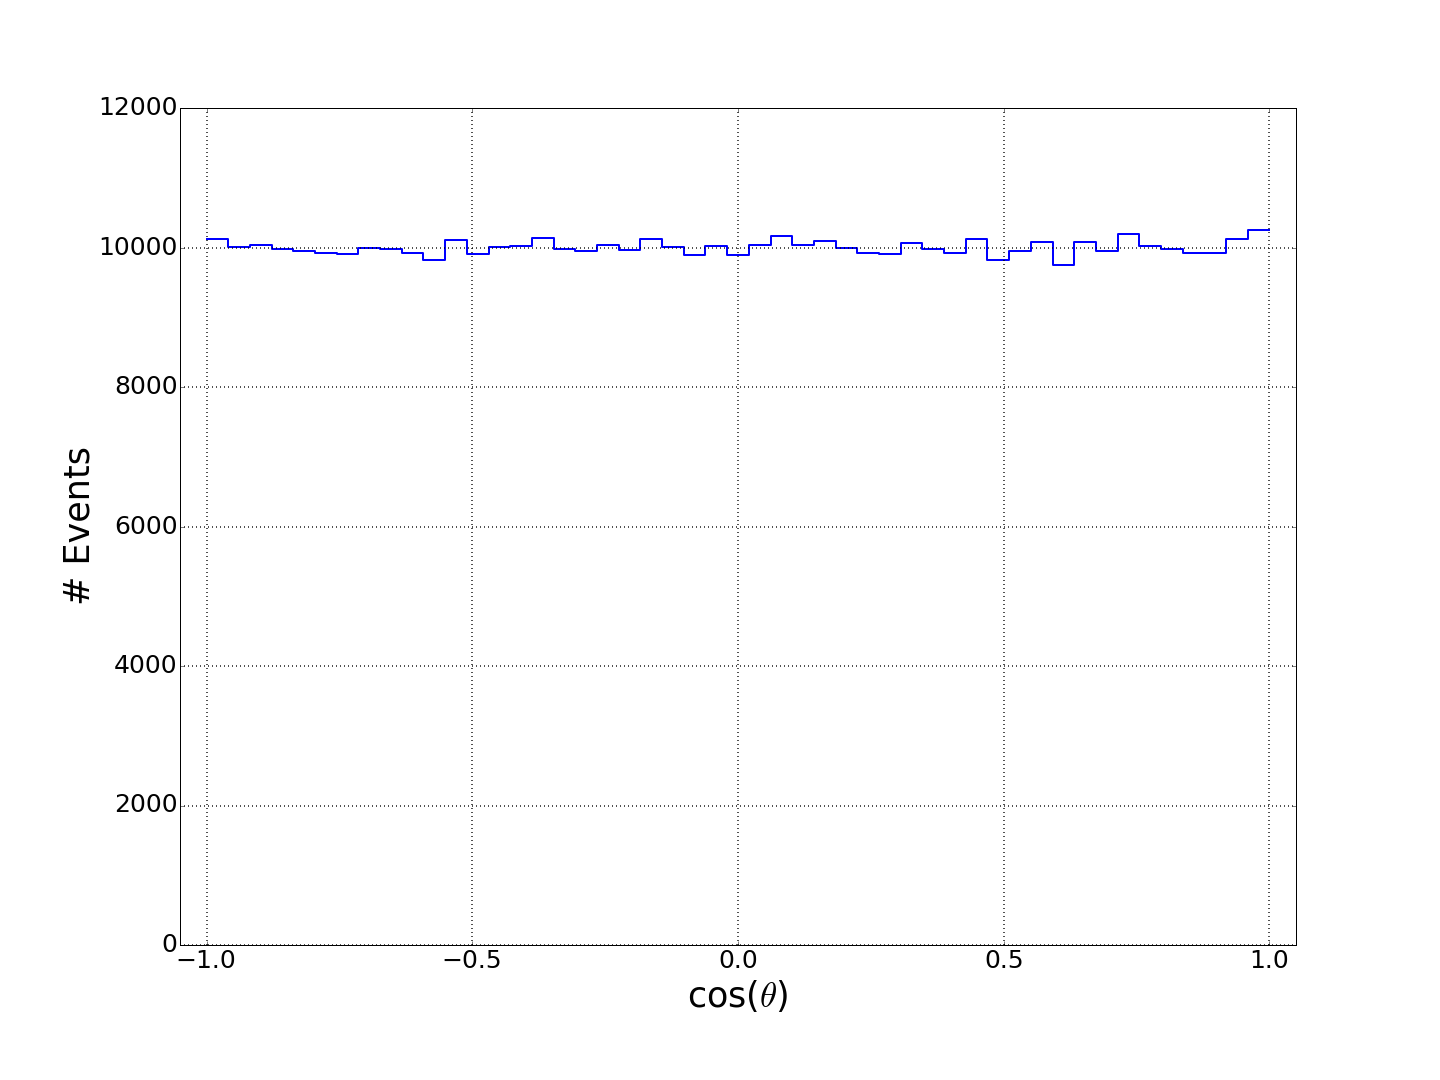
\includegraphics[width=0.49\textwidth]{chapter6/img/Zenith_full}
\caption{Illustration of uniform distributions of azimuth and cosine of the zenith for the particle injection in agreement with an isotropic flux (see Appendix \ref{sec:sphericalrandom}). The zenith angle in this example ranges from 0$^\circ$ to 86$^\circ$ }.
\label{fig:angles}
\end{figure}

\noindent Because slow moving particles would require specialized treatment\footnote{Cherenkov photon production in Eq. \ref{eq:franktamm} changes for $\beta < 1$ compared to relativistic particles ($\beta \approx 1$). Similarly, ionization effects as seen in Eq. \ref{eq:ioniz} for slow moving particles would not be comparible to relativistic particles. Also, the IceCube detector is designed to trigger on relativistic particles and most of the cleaning tools (see Section \ref{sec:pulsecleaning}) rely on relativistic speeds. Dedicated analyses on slow moving particles like monopoles are being done but need specialized simulation and analyses. This is beyond the scope of this work.}, therefore, the minimal velocity of the particles is set as $\beta > 0.95$. The energy distribution is simulated with an $E^{-1}$ spectrum and is later normalized to a flux of $10^{-14} \textrm{ GeV } \textrm{cm}^{-2} \textrm{ s}^{-1} \textrm{ sr}^{-1}$ with an $E^{-2}$ spectrum (see Appendix \ref{sec:powerlawdistr}) where the absolute flux is only necessary for illustrative purposes (see Section \ref{subsec:mrf}).\\

\noindent Similar to the background, SpiceLea was used as the nominal ice model.

\section{Propagation}
After generation, the particles need to be propagated through the ice. The particles will interact, lose energy, produce new particles, and generate light. The particle interactions and light production are done in two different modules. The former module is called \texttt{PROPOSAL} and runs on normal CPUs, whereas the latter is called \texttt{ppc} and uses GPUs to simulate enormous amounts of photons that are propagated through the ice.


\subsection{\texttt{PROPOSAL}}
Using the cross sections of the important interactions, together with the properties of the traversed medium and the particles (mass, charge, spin, decay time, etc.), it is possible to simulate the energy losses, secondary production and the consequent interactions of these daughter particles. This is done in the software package \texttt{PROPOSAL} \index{PROPOSAL} (the Propagator with Optimal Precision and Optimized Speed for All Leptons), fully written in C++. It was based on its predecessor \texttt{MMC} (Muon Monte Carlo), which was written in Java. In 2018, a substantially improved version of \texttt{PROPOSAL} was finalized. An illustration of the workings of the code is given in Figure \ref{fig:proposal} and an in-depth documentation is given in Ref. \cite{Dunsch:2018nsc}.

\paragraph{\texttt{PROPOSAL} for SMPs}
Since we assume the SMPs to behave leptonically, it was chosen to use \texttt{PROPOSAL} for the signal propagation as well. The mass and charge of the particle are set in the input parameters and the cross section dependence on these parameters can be seen in Section \ref{sec:energyloss}. In general, there is a small dependence on the mass and a dependence on the square of the charge, except for bremsstrahlung, which has a quartic charge dependence.

\begin{figure}
\centering
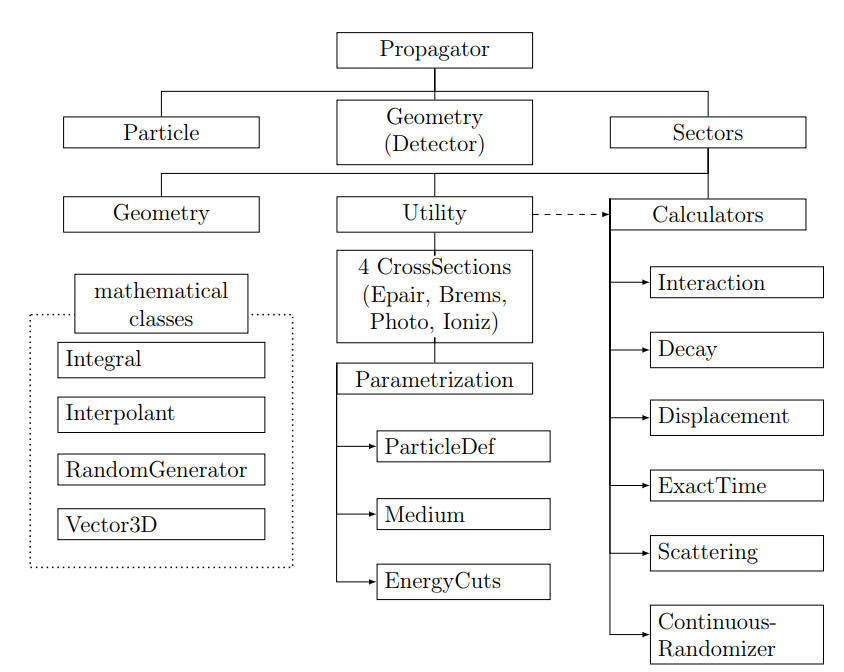
\includegraphics[width=0.7\textwidth]{chapter6/img/proposal.png}
\caption{Overview of the class structure in \texttt{PROPOSAL}, from Ref. \cite{Dunsch:2018nsc}.}
\label{fig:proposal}
\end{figure}

\noindent The \texttt{PROPOSAL} module keeps track of all the particles that are produced during propagation and the accompanying energy losses in a tree-like structure (called an \textit{I3MCTree}). This collection of particles and their interactions are forwarded to a light-production computation module.

\subsection{Photoelectron generators}
In Section \ref{subsec:icesimulation} we already explained how the ice is simulated in the IceCube detector. The parameters $b_e(400)$ and $a_{dust}(400)$ define the photon propagation through the ice and determine if photons are absorbed in the ice or hit a DOM. To optimize computing time, the DOMs were scaled in radius (nominally with a factor of 5) to force more photon interactions. The number of photons emitted was then appropriately scaled down with the square of this scaling factor\footnote{The surface of a sphere scales with the square of the radius.}. With the Frank-Tamm formula (Eq. \ref{eq:franktamm}) it is possible to calculate the expected number of photons produced per unit length in the wavelength interval of interest\footnote{From Figure \ref{fig:acceptance} it is clear that $\lambda_1 \approx 300$ nm and $\lambda_2 \approx 650$ nm.}

\begin{equation}
\frac{dN}{dx} = \int_{\lambda_1}^{\lambda_2} \frac{2 \pi \alpha}{\lambda^2} \sin^2 \left(\theta_c\right) d\lambda = 2\pi \alpha \sin^2 \left(\theta_c\right) \left(\frac{1}{\lambda_1} -\frac{1}{\lambda_2}\right).
\end{equation}
From this formula, we find that the expected rate of a Cherenkov emission profile is equal to $\approx 350$ photons/cm. Together with the DOM acceptance curve, as shown in Figure \ref{fig:acceptance}, which has an overall average of around 7\%, the expected \textit{observed} number of photons is equal to 2450 m$^{-1}$.\\

\noindent \texttt{PPC}\index{PPC} is a Photon Propagation Code, written in C++ that runs on graphic processing units (GPUs). This allows the code to run up to a hunderd times faster than in a CPU-only environment. \texttt{PPC} employs both CUDA (NVIDIA GPU only) and OpenCL programming interface (both NVIDIA and AMD GPUs) together with multiple CPU environments.
GPU environments allow the tracking of thousands of photons simultaneously, vastly improving the computational speed. For more information, see Ref. \cite{dimaspice}.

Previous photon propagation codes, such as \texttt{Photonics} \index{Photonics} \cite{Lundberg:2007mf}, produced 6-dimensional photon tables (3 spatial, 2 directional and 1 temporal). This meant that at least one set of tables had to be produced per particle type and per velocity and interpolation methods had to be used, with the accompanying inaccuracies. These tables also required significant disk space and the method was therefore replaced with the GPU-codes. Direct photon simulation also allows for other non-trivial implementations such as the tilting of ice layers.\\

\noindent Another photon propagation code is called \texttt{CLSim}\index{CLSim}, which uses GEANT4 to propagate particles. A hybrid version called \texttt{HybridCLsim} is often used. Muons are propagated using \texttt{PROPOSAL}/\texttt{MMC} \index{MMC} and their stochastic losses (which are small showers) are simulated from tables whereas the ``bare muons'' (with their stochastics) are simulated using direct propagation. This avoids time loss for the rare but very computational high-energy cascade events.\\

\noindent An illustration of photon propagation in the IceCube detector for both a cascade and track simulation is shown in Figure \ref{fig:photonsimulation}.

\begin{figure}
\centering
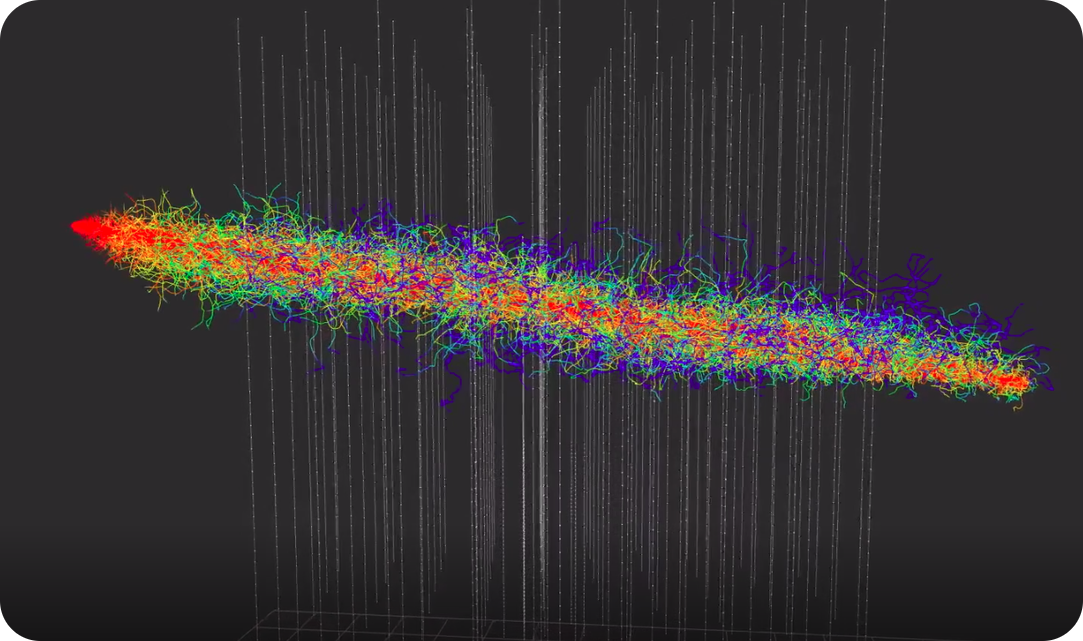
\includegraphics[width=0.8\textwidth,height=2.6in]{chapter6/img/photons_track_rounded.png}
%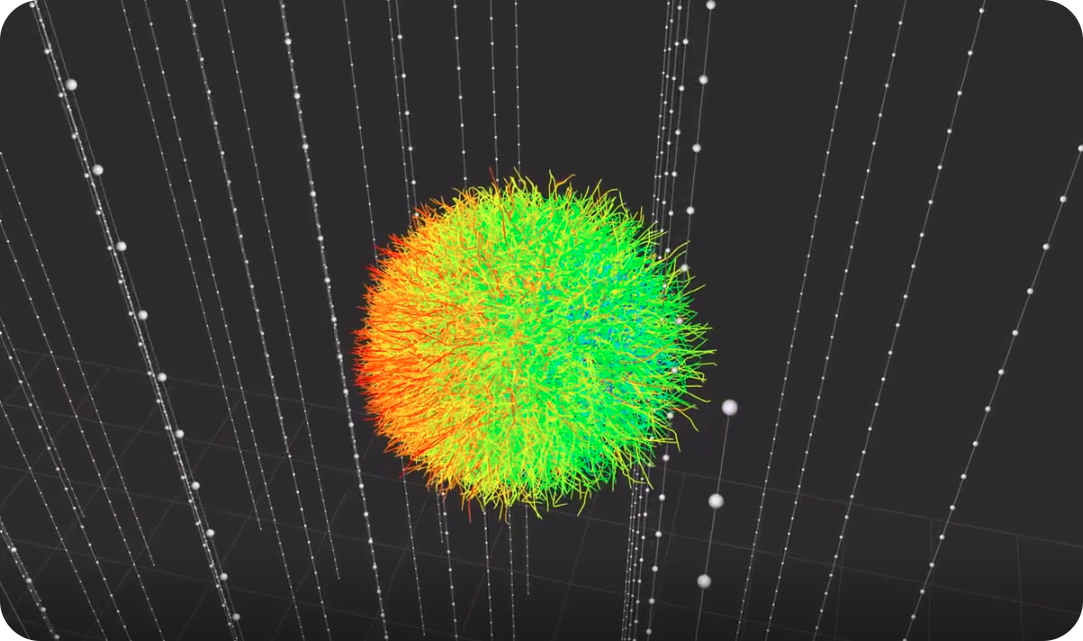
\includegraphics[width=0.48\textwidth,height=1.9in]{chapter6/img/photons_cascade_rounded.png}
\caption{\textit{Left:} simulation of a track event in IceCube. Each line represents a photon path and colors indicate how far they have traveled from their generation point. \textit{Right:} simulation of a cascade event in IceCube.}
\label{fig:photonsimulation}
\end{figure}
%Hier ook indirect cherenkov light component

\textcolor{red}{\\Nergens vermeldt hoe je je signaal verandert hebt hierop...\\}

\section{Detector simulation}
Further processing of the simulations involve:
\begin{itemize}
\item \texttt{Polyplopia}: a project dedicated to merge multiple events to account for coincident events (that are simulated independently). An estimated 15\% of CORSIKA events result in coincident events and make up de bulk of bad reconstructions where down-going muons are simulated as up-going (example see Figure \ref{fig:coincidentevent});
\item \texttt{Vuvuzela}: the PMT noise is simulated as having an exponential component from  thermal and radioactive decays, and a log-normal contribution for scintillation;
\item \texttt{PMT}: the time from the first photon entering the PMT to the readout after passing along multiple dynodes has an uncertainty, referred to as ``PMT jitter''\index{PMT jitter}. The amplification of photoelectrons by the PMT is also not constant and is simulated in this module. Additionally, the module accounts for prepulses, late pulses, afterpulses and saturation of the PMT. More information can be found in Refs. \cite{Abbasi:2010vc,Ma:2009aw}.
\item \texttt{DOMLauncher}: the digitization of the PMT pulses and other behavior of the DOM mainboard (as explained in Section \ref{subsec:mainboard}) is done in this module. The three main features of the DOM that are simulated to generate launches are the discriminator, LC, and digitization.
\item \texttt{trigger-sim}: simulation of the trigger behavior as explained in Sec. \ref{subsec:triggers}.
\end{itemize}

\section{Processing}
\label{sec:processing}
After a full particle propagation and detector response simulation, the sample is sent through the same PnF procedure as is done with the data (see Section \ref{subsec:filters}). The different stages of processing are referred to as ``Levels'', where basic conversion from PnF formats to i3files (see Section \ref{subsec:datahandling}) is called \textit{Level0}. Reconstructions, calibrations and hit cleaning necessary for the filters are done at \textit{Level1} while the filter processing is done at \textit{Level2} (Section \ref{subsec:filters}).

\section{Simulation validation: burn sample}
\label{sec:burnsample}
Getting the intricate details of physical events in non-trivial environments just right is not an easy task. In many steps of the way, simulations use fits and estimations. Some simulation datasets are reasonable to compare to the data, depending on the phase space one is looking at, while other datasets need other specifications. For example, analyses dedicated to measuring the cosmic ray interactions need much more fine-tuning in their models for the atmosphere, composition, interaction models, etc. than an analysis dedicated to search for muon tracks that first propagated through the Earth and have atmospheric muons as a background. Similarly, in this analysis the burn sample was used to compare data and MC to determine if the agreement between both made for a valid comparison. This is done in the analysis presented in Chapter \ref{ch:space}.

It is for this reason that most analyses select a certain subset of the data they want to analyze to compare to the Monte Carlo simulations. For the present work, 10\% of the total data, called the \textit{burn sample}\index{burn sample}, was used to compare data to Monte Carlo. As indicated in Section \ref{subsec:datahandling}, the data is saved in 8 hour runs and the burn sample consists of every run that ends on a `0'. The burn sample also allows to estimate the robustness of certain reconstructions and variables regarding differences in data and simulation.\\

\noindent After the discovery of an SPE offset in the DOM response in 2015, it was decided that multiple years of data was to be reprocessed in what was called \textit{pass2 reprocessing} \cite{pass2}. Aside from the SPE correction, the raw pulses were reprocessed with 2017 PnF, making the data more uniform in the course of the years for easier comparison\footnote{Most filters did not undergo changes or only minor ones.}. This analysis makes use of data starting in the years 2011 to 2015 and are referred to as IC86-1 to IC86-5 where IC86 stands for the complete 86-string IceCube detector configuration and the last digit refers to the year of the season start. More recent years were not fully processed in time for this analysis. Only runs were considered that had
\vspace{2mm}
\begin{enumerate}
\item a positive tag from run coordinators (status == ``good\_i3''),
\item at least 5000 active optical modules,
\item all strings active during runtime.
\end{enumerate}
\vspace{2mm}

\noindent The \textit{livetime} is the total time that the detector was up and running and non-corrupted data was processed. Due to the increase in detector uptime over the years, this also means that the livetime of the different datasets has increased. The livetime for the different years is equal to
\vspace{2mm}
\begin{itemize}
\item around 31 days of livetime for IC86-1,
\item around 32.2 days of livetime for IC86-2,
\item around 33.2 days of livetime for IC86-3,
\item around 36.6 days of livetime for IC86-4,
\item around 36.7 days of livetime for IC86-5,
\end{itemize}
\vspace{2mm}

\noindent resulting in a total burn sample livetime of around 170 days.

\textcolor{red}{In tabel misschien? En data van start/einde...?}

\section{Event viewer}
After a full simulation, it is possible to visualize the event in an event viewer called \texttt{Steamshovel}\index{Steamshovel}. Typical events in the IceCube detector are shown with this interface and are loaded from \textit{i3files} that contain information about the detector geometry and the full event (DOM positions and calibrations, detector hits, timestamps, trigger hits, etc.). Simulated events also contain the true values of the particles and can be compared with reconstructed variables. Event viewers allow for first guesses in how background events are able to be separated from signal, although both can have wide varieties in possible outputs.

The number of photons seen per DOM is indicated by the size of the spheres; the larger the sphere, the more PEs were seen. The color of the modules indicates the time of the pulse registration. The color scale can be chosen, but usually a rainbow pattern is used where red indicates the earliest pulse hits and blue the last. 

An example of a track event in the event viewer is given in Figure \ref{fig:photonsimulation}.